\def\sgn{\mathrm{sgn}}
\def\adj{\mathrm{adj\ }}

\section{Determinanty}

\begin{pozadavky}
\begin{pitemize}
\item Definice a základní vlastnosti determinantu
\item Úpravy determinantů, výpočet
\item Geometrický smysl determinantu
\item Minory a inversní matice
\item Cramerovo pravidlo.
\end{pitemize}
\end{pozadavky}

\subsection{Definice a základní vlastnosti determinantu}

\begin{obecne}{Neformálně}
V lineární algebře je \emph{determinant} zobrazení, které přiřadí každé čtvercové matici $A$ skalár $\det A$.

Determinantem čtvercové matice řádu $n$ nazýváme součet všech součinů $n$ prvků této matice takových, že v žádném z uvedených součinů se nevyskytují dva prvky z téhož řádku ani z téhož sloupce. Každý součin přitom násobíme čísly $r$ a $s$, kde $r$ představuje znaménko permutace příslušného pořadí prvních indexů a $s$ znaménko permutace příslušného pořadí druhých indexů.
\end{obecne}

\begin{definiceN}{permutace, znaménko}
\emph{Permutace} je libovolná bijekce $\sigma:X\to X$. Množina \emph{inversí} nějaké permutace $\sigma$ je $I(\sigma)=\{(i,j):i<j \ \&\ \sigma(i)>\sigma(j)\}$. Znaménko permutace $\sgn(\sigma)$ se pak definuje jako $\sgn(\sigma)=(-1)^{|I(\sigma)|}$. Nejjednodušší permutace -- záměna dvou prvků -- se pak nazývá \emph{transpozice}. Ta má vždy znaménko $-1$ a libovolná permutace je složením nějakých transpozic. Množinu všech permutací na množině $\{1,\dots,n\}$ značíme $S_n$.
\end{definiceN}

\begin{poznamka}
Pro skládání permutací platí $\sgn(p\circ q)=\sgn(p)\sgn(q)$. Pro inversní permutaci (inversní zobrazení) platí $\sgn(p)=\sgn(p^{-1})$.
\end{poznamka}

\begin{definiceN}{determinant}
Nechť $A = (a_{i,j})^{n}_{i,j=1}$ je čtvercová matice řádu $n$.
Determinant je definovaný pomocí \emph{Leibnizova vzorce}:

$$\det A = \sum_{\sigma \in S_n}sgn(\sigma) \prod_{i=1}^n a_{i,\sigma(i)}$$
\end{definiceN}

\begin{poznamka}
Suma se počítá přes všechny permutace $\sigma$ čísel \{1,2,\dots,n\}, takže tento vzorec obsahuje $n!$ (faktoriál) sčítanců, což jej s růstem \emph{n} rychle činí prakticky nepoužitelným pro výpočet. V praxi se proto používají jiné způsoby výpočtu.
\end{poznamka}

\begin{poznamka}
Konkrétně, pro matici řádu $n$, kde:
\begin{pitemize}
\item $n=1: \det A = a_{1,1}$
\item $n=2: \det A = a_{1,1} a_{2,2} - a_{2,1} a_{1,2}$
\item $n=3: \det A = a_{1,1} a_{2,2} a_{3,3} + a_{1,3} a_{2,1} a_{3,2} + a_{1,2} a_{2,3} a_{3,1} - a_{1,3} a_{2,2} a_{3,1} - a_{1,1} a_{2,3} a_{3,2} - a_{1,2} a_{2,1} a_{3,3}$
\end{pitemize}

Mnemotechnická pomůcka sloužící k zapamatování postupu výpočtu determinantu třetího řádu se nazývá \emph{Sarrusovo pravidlo}:
\begin{center} 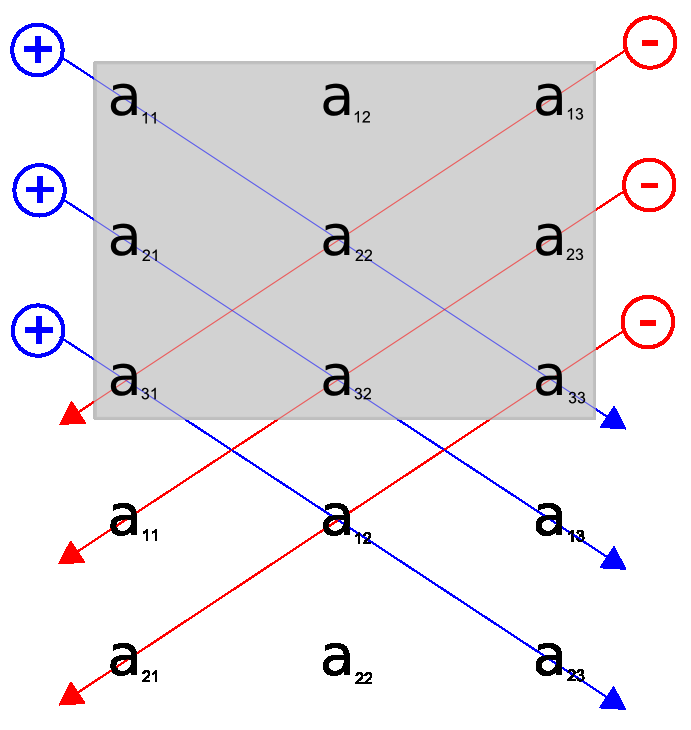
\includegraphics[width=5cm]{matematika/obrazky/sarrusovo_pravidlo.png} \end{center}
\end{poznamka}

\begin{poznamka}
Obecný vzorec lze také vyjádřit pomocí Levi-Civitova symbolu $\epsilon_{{j_1}{j_2}\dots{j_n}}$ jako
$$\det A = \sum_{{j_1},{j_2}, \dots ,{j_n}}\epsilon_{{j_1}{j_2} \dots {j_n}} a_{1,j_1}a_{2,j_2}  \dots  a_{n,j_n} = \sum_{{j_1},{j_2}, \dots ,{j_n}}\epsilon_{{j_1}{j_2} \dots {j_n}} a_{j_1,1}a_{j_2,2}  \dots  a_{j_n,n}$$
\end{poznamka}

\subsubsection*{Vlastnosti determinantu}

\begin{vetaN}{O determinantu transponované matice}
Pro čtvercovou matici $A$ řádu $n$ platí:
$$\det A=\det A^T$$

\begin{dukaz}
Plyne z faktu že $\sgn(p)=\sgn(p^{-1})$:
\begin{align*}
\det(A^T) & =\sum_{p\in S_n}\sgn(p)\prod_{i=1}^n(A^T)_{i,p(i)}=\\
 & =\sum_{p\in S_n}\sgn(p)\prod_{i=1}^n a_{p(i),i}=\sum_{p^{-1}\in S_n}\sgn(p^{-1})\prod_{i=1}^n a_{i,p^{-1}(i)}=\det(A)
\end{align*}
\end{dukaz}
\end{vetaN}

\begin{vetaN}{Přerovnání matice}
Přerovnání řádků nebo sloupců podle permutace $p$ nezmění determinant vůbec, pokud $\sgn(p)=1$ a změní jen jeho znaménko, pokud $\sgn(p)=-1$.

\begin{dukaz}
A buď původní matice a B přerovnaná:
\begin{align*}
\det(B) & =\sum_{p\in S_n}\sgn(p)\prod_{i=1}^n(B)_{i,p(i)} = \sum_{p\in S_n}\sgn(p)\prod_{i=1}^n(A)_{i,q^{-1}\left(p(i)\right)}=\\
 & =\sgn(q)\sum_{p\in S_n}\sgn(q)\sgn(p)\prod_{i=1}^n(A)_{i,q^{-1}\left(p(i)\right)}=\sgn(q)\sum_{p\in S_n}\sgn(h)\prod_{i=1}^n(A)_{i,h(i)}=\\
 & =\sgn(q)\det(A)
\end{align*}
\end{dukaz}
\end{vetaN}

\begin{dusledek}
Má-li matice dva shodné sloupce nebo řádky, má automaticky nulový determinant (přehozením právě těch dvou řádků nebo sloupců vzniknou shodné matice se stejným determinantem, ale má se změnit znaménko).
\end{dusledek}

\begin{vetaN}{Determinant jako lineární funkce}
Determinant matice $A$ je lineární funkcí každého jejího řádku i každého sloupce, tj. platí
\begin{penumerate}
    \item $$\det\left(\begin{matrix}
a_{1,1}& \dots & a_{1,n}\\
\vdots & & \vdots \\
b_{i,1}& \dots & b_{i,n}\\
\vdots & & \vdots \\
a_{n,1}& \dots & a_{n,n}\\
\end{matrix}\right)
+ \det\left(\begin{matrix}
a_{1,1}& \dots & a_{1,n}\\
\vdots & & \vdots \\
c_{i,1}& \dots & c_{i,n}\\
\vdots & & \vdots \\
a_{n,1}& \dots & a_{n,n}\\
\end{matrix}\right)
= \det\left(\begin{matrix}
a_{1,1}& \dots & a_{1,n}\\
\vdots & & \vdots \\
b_{i,1} + c_{i,1}& \dots & b_{i,n} + c_{i,n}\\
\vdots & & \vdots \\
a_{n,1}& \dots & a_{n,n}\\
\end{matrix}\right)$$
    \item $$\det\left(\begin{matrix}
a_{1,1}& \dots & a_{1,n}\\
\vdots & & \vdots \\
\kappa a_{i,n}& \dots & \kappa a_{i,n}\\
\vdots & & \vdots \\
a_{n,1}& \dots & a_{n,n}\\
\end{matrix}\right)
= \kappa \det(A)$$
\end{penumerate}

\begin{dukaz}
První část plyne z distributivity sčítání vzhledem k násobení -- každý člen sumy (produkt prvků) obsahuje jeden prvek typu $b_{i,p(i)} + c_{i,p(i)}$ pro nějakou permutaci a ten je možné rozepsat. Druhá část se dokáže podobně díky komutativitě násobení -- prvek $\kappa$ je také obsažen v každém členu sumy právě jednou, takže je ho možné \uv{vytknout}.
\end{dukaz}
\end{vetaN}

\begin{vetaN}{Determinant součinu matic}
Nechť $A$ a $B$ jsou čtvercové matice stejného řádu $n$ nad tělesem $T$. Potom platí:
$$\det(A\cdot B)=\det(A)\cdot\det(B)$$

\begin{dukaz}
Je-li jedna z matic singulární, je jejich součin singulární a tedy má nulový determinant; stejně jako je nulový součin determinantů původních matic. Jsou-li obě matice regulární, lze $A$ rozložit na nějaký součin $E_1\cdot E_2\cdot\dots\cdot E_k$ elementárních matic. Potom 
\begin{align*}
\det(AB) & = \det(E_1E_2\dots E_k B)=\det(E_1)\cdot\det(E_2\dots E_k B)\\
& =\det(E_1)\det(E_2)\dots\det(E_k)\det(B)=\det(A)\det(B)
\end{align*}
protože víme, jakým způsobem elementární úpravy (ekvivalent elementárních matic ve vzorci) mění determinant.
\end{dukaz}
\end{vetaN}

\begin{dusledek}
Čtvercová matice je regulární, právě když má nenulový determinant.
\end{dusledek}

\subsection{Úpravy determinantů, výpočet}

\begin{obecne}{Gaussova eliminace}
Gaussova metoda spočívá v provedení takových úprav matice, které nemění hodnotu determinantu, ale zjednoduší výpočet jeho hodnoty. Cílem prováděných úprav je získat trojúhelníkovou matici \textbf{A} (kde pro $i > j$ je $a_{i,j} = 0$), neboť pro trojúhelníkové matice platí

$$\det A = a_{1,1} a_{2,2}  \dots  a_{n,n}$$

\noindent
tzn. determinant je roven součinu prvků hlavní diagonály matice.

\noindent
Při úpravách matice pro výpočet determinantu postupujeme podle těchto pravidel:
\begin{pitemize}
\item Pokud \textbf{B} vznikne z \textbf{A} výměnnou dvou řádku nebo sloupců potom $\det B = -\det A$
\item Pokud \textbf{B} vznikne z \textbf{A} vynásobením řádku nebo sloupce skalárem c, potom $\det B = c.\det A$
\item Pokud \textbf{B} vznikne z \textbf{A} přičtením násobku jednoho řádku k jinému, nebo přidáním násobku sloupce k jinému sloupci potom $\det B = \det A$
\end{pitemize}

\noindent
Opakovaným použitím uvedených pravidel převedeme matici na trojúhelníkovou a pro tu poté snadno spočteme determinant.
\end{obecne}



\subsection{Geometrický smysl determinantu}

\begin{obecne}{Matice řádu 2}
Absolutní hodnotu determinantu matice řádu 2
$$\det\left(
\begin{array}{cc}
a & b\\
c & d
\end{array}
\right) = ad - bc
$$
lze interpretovat jako obsah rovnoběžníku s vrcholy v bodech $(0,0)$, $(a,c)$, $(b, d)$ a $(a+b, c+d)$. Znaménko determinantu určuje vzájemnou orientaci vektorů $(a,c)$, $(b, d)$. $\det A$ je kladný, pokud úhel mezi vektory $(a,c)$, $(b, d)$ měřený v kladném směru (tedy proti směru hodinových ručiček) menší než $\pi$, a záporný, pokud je tento úhel větší než $\pi$.
\end{obecne}

\begin{obecne}{Matice řádu 3}
Podobný geometrický význam jako pro matici řádu 2 najdeme i pro matice $B = (b_{i,j})$ řádu 3. Řádkové vektory

$$b_1 = (b_{1,1}, b_{1,2}, b_{1,3}), b_2 = (b_{2,1}, b_{2,2}, b_{2,3}), b_3 = (b_{3,1}, b_{3,2}, b_{3,3})$$

určují v třídimenzionálním prostoru rovnoběžnostěn, jehož objem je roven $\left| \det B \right|$. Pokud je $\det B$ kladný, tak je posloupnost vektorů $b_1, b_2, b_3$ pravotočivá, a levotočivá, pokud je $\det B$ záporný.
\end{obecne}

\begin{obecne}{Matice vyšších řádů}
I v reálných prostorech vyšších řádů lze determinant chápat jako objem obecného \emph{n}-rozměrného rovnoběžnostěnu, případně jako pravotočivost, respektive levotočivost posloupnosti $b_1, b_2,  \dots , b_n$.
\end{obecne}

\begin{definiceN}{Pravotočivá a levotočivá soustava prostorových kartézských souřadnic}
Představte si, že v místě, kde stojíte, je počátek prostorové kartézské soustavy. Osa x nechť směřuje přímo vpřed (směrem, kterým se díváte), osa y nechť směřuje vlevo a osa z nechť směřuje vzhůru. Taková soustava se nazývá \emph{pravotočivá souřadná soustava}.

Zaměníme-li osy x a y, získáme \emph{souřadnou soustavu levotočivou}. Obvykle se pracuje s pravotočivou souřadnou soustavou.

Mnemotechnická pomůcka: Soustava souřadnic je pravotočivá pokud při naznačení kladného směru osy z zdviženým palcem pravé ruky naznačují ostatní prsty směr od kladného směru osy x ke kladnému směru osy y.
\end{definiceN}


\subsection{Minory a inversní matice}

\begin{definiceN}{Minor}
Mějme čtvercovou matici $A_{ij}$, kterou získáme z matice $A$ odstraněním i-tého řádku a j-tého sloupce. Determinant matice $A_{ij}$, tzn. $\det A_{ij}$ nazýváme \emph{subdeterminantem} (též \emph{minorem}) příslušným k prvku $a_{i,j}$ matice $A$.
\end{definiceN}

\begin{obecne}{Výpočet determinantu rozvojem podle řádků (sloupců)}
Algebraický doplněk lze použít k výpočtu determinantu \emph{n}-tého řádu. Pro libovolné (pevně dané) \emph{i} lze determinant matice $A$ vyjádřit pomocí algebraických doplňků jako

$$\det( A ) = \sum_{j=1}^n a_{i,j}\cdot (-1)^{i+j}\det( A_{ij} )$$

Tento postup je označován jako \emph{rozvoj (rozklad) determinantu podle i-tého řádku}. Ekvivalentně lze determinant vyjádřit \emph{rozvojem (rozkladem) podle j-tého sloupce}. Číslo $(-1)^{i+j}\det( A_{ij} )$ se někdy nazývá \emph{kofaktorem} nebo \emph{algebraickým doplňkem}.
\end{obecne}

\begin{definiceN}{Adjungovaná matice}
Pro čtvercovou matici $A$ definujeme \emph{adjungovanou matici} $\adj A$ předpisem
$$(\adj A)_{i,j}=(-1)^{i+j}\cdot\det(A_{ji})$$
kde $A_{ji}$ jsou minory matice $A$ (s vynechaným $j$-tým řádkem a $i$-tým sloupcem -- pozor na obrácené pořadí indexů!). Prvky adjungované matice jsou vlastně algebraické doplňky v transponované matici $A^T$.
\end{definiceN}

\begin{definiceN}{Inversní matice}
Pro čtvercovou matici $A$ řádu $n$ definujeme inverzní matici $A^{-1}$ předpisem
$$A.A^{-1} = A^{-1}.A = I_n$$
kde $I_n$ je jednotková matice. Inversní matici lze sestrojit pouze pro regulární matici.
\end{definiceN}

\begin{vetaN}{Výpočet inversní matice podle minorů}
Pro každou regulární matici $A$ nad tělesem $T$ platí: 
$$A^{-1}=\frac{1}{\det A}\cdot(\adj A)$$
$$A^{-1}_{i,j}=(-1)^{i+j}\frac{\det(A_{ji})}{\det A}$$

\begin{dukaz}
Z maticového součinu $A\cdot\adj A$:
\begin{penumerate}
    \item $i$-tý řádek $A$ $\times$ $i$-tý sloupec $\adj A$ (obs. determinanty minorů odp. $i$-tému řádku) dá dohromady $\det A$
    (z rozvoje determinantu podle řádku)
    \item $j$-tý řádek $A$ $\times$ $i$-tý sloupec $\adj A$ dá dohromady $0$, protože jde o stejný princip pro matici, kde $i$-tý
    řádek je nahrazen $j$-tým (2 stejné řádky)
\end{penumerate}
Potom $A\cdot\adj A = \det A\cdot I_n$ a to už dává $\frac{1}{\det A}\adj A = A^{-1}$.
\end{dukaz}
\end{vetaN}


\subsection{Cramerovo pravidlo}
Cramerovo pravidlo je metoda umožňující nalezení řešení soustavy lineárních algebraických rovnic.

\begin{obecne}{Postup}
Mějme soustavu lineárních rovnic, která obsahuje stejný počet neznámých jako je počet rovnic. Označme matici soustavy $A$. Dále označme $A_i\;$ jako matici, kterou získáme z matice $A$, nahradíme-li v ní $i$-tý sloupec sloupcem pravých stran soustavy rovnic.

Pokud zapíšeme matice soustavy a vektor pravých stran jako

$$
A =
\left( \begin{array}{cccc}
    a_{11} & a_{12} & \dots  & a_{1n} \\
	a_{21} & a_{22} &  \dots  & a_{2n} \\
	\vdots  &  \vdots  &  \ddots  &  \vdots \\
	a_{m1} & a_{m2} &  \dots  & a_{mn}
\end{array} \right), 
B = \left( \begin{array}{cccc} b_1 \\b_2 \\ \vdots  \\b_m \end{array} \right)
$$

pak má tvar

$$
A_i=
\left( \begin{array}{cccccccc}
	a_{11} & a_{12} & \dots & a_{1,i-1} & b_1 & a_{1,i+1} & \dots  & a_{1n} \\
	a_{21} & a_{22} & \dots & a_{2,i-1} & b_2 & a_{2,i+1} & \dots  & a_{2n} \\
	\vdots & \vdots & \vdots & \vdots & \vdots & \vdots & \ddots & \vdots \\
	a_{m1} & a_{m2} & \dots & a_{m,i-1} & b_m & a_{m,i+1} & \dots & a_{mn}
\end{array} \right)
$$

Pokud je determinant matice soustavy nenulový, $\det A \neq 0$, tzn. matice je regulární, pak má soustava právě jedno řešení, pro které platí

$$x_i = \frac{\det A_i}{\det A}$$

pro $i = 1,2, \dots ,n$.
\end{obecne}

\begin{dukaz}
Pro soustavu $Ax=b$ -- rozepíšeme $x=A^{-1}b$, ze vzorce pro inversní matici plyne
$$x=\frac{1}{\det A}(\adj A)\cdot b$$
takže pro $x_i$ vychází 
$$x_i=\frac{1}{\det A}((\adj A)b)_i=\frac{1}{\det A}\cdot\sum_{j=1}^n(\adj A)_{i,j}\cdot b_j=\frac{1}{\det A}\cdot\det A_i$$
\end{dukaz}

\begin{priklad}
Úkolem je řešit soustavu rovnic
 $$x + y = 3$$
 $$x - 2y = 1$$

Determinant matice soustavy je
 $$\det A = \left| \begin{array}{cc}1 & 1 \\ 1 & -2\end{array} \right| = -3$$

Poněvadž je $\det A \neq 0$, lze použít Cramerovo pravidlo.

Dále určíme
 $$\det A_1 = \left| \begin{array}{cc}3 & 1 \\ 1 & -2\end{array} \right| = -7$$
 $$\det A_2 = \left| \begin{array}{cc}1 & 3 \\ 1 & 1\end{array} \right| = -2$$

Řešení má tedy tvar
 $$x = \frac{\det A_1}{\det A} = \frac{-7}{-3} = \frac{7}{3}$$
 $$y = \frac{\det A_2}{\det A} = \frac{-2}{-3} = \frac{2}{3}$$

Zkouškou se přesvědčíme, že se skutečně jedná o řešení uvedené soustavy.
\end{priklad}
